\section*{Results}

\subsection*{Experiment Loss and Accuracy}

Here are the test loss and accuracy of each experiment.

\begin{table}[H]
    \centering
    \begin{tabular}{|c|l|l|l|}
        \hline
        Exp. Index & Experiment & Loss & Accuracy \\
        \hline
        1 & Test set before fine-tuning    & 765.904 & 0.009751 \\
        \hline
        2 & Test set after fine-tuning     & 167.609 & 0.858439 \\
        \hline
        3 & Test set with first technique  & 134.134 & 0.876086 \\
        \hline
        4 & Test set with second technique & 122.907 & 0.885339 \\
        \hline
        5 & Test set with two techniques   & 123.766 & 0.886012 \\
        \hline
        6 & Test set with SupContrast      & 33.681 & 0.879623 \\
        \hline
        7 & Test set with SimCLR           & 46.681 & 0.868623 \\
        \hline
    \end{tabular}
    \vspace{2mm}
    \caption{Experimental Results}
    \label{tab:exp}
\end{table}

\subsection*{Accuracy Plots}

Here are the accuracy plot of the 5 models.

\begin{figure}[H]
    \centering
    \subfloat[\centering Basline Accuracy]
    {{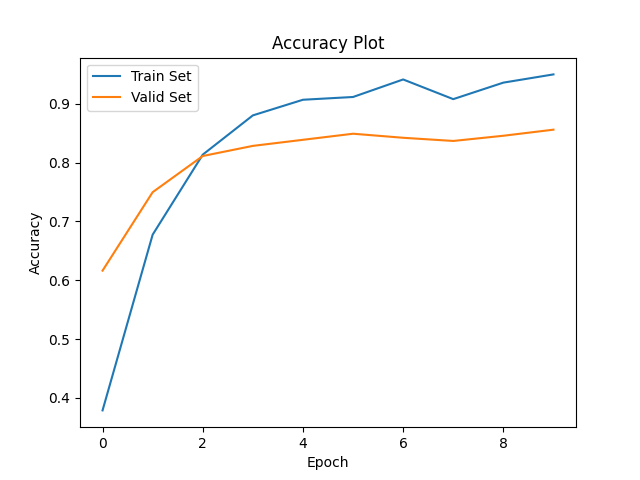
\includegraphics[scale=0.3]{./plots/baseline_10_Accuracy.png} }}
    \subfloat[\centering Technique One Accuracy]
    {{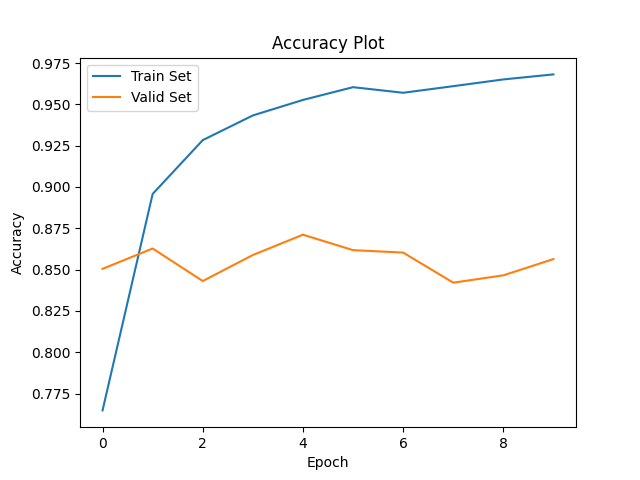
\includegraphics[scale=0.3]{./plots/tune1_10_Accuracy.png} }}
    \subfloat[\centering Technique Two Accuracy]
    {{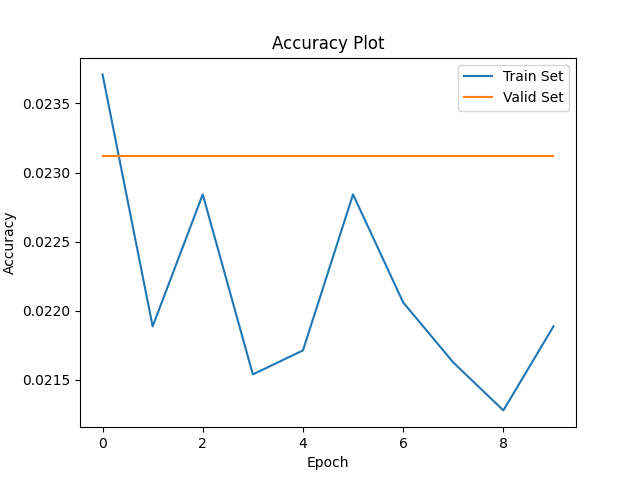
\includegraphics[scale=0.3]{./plots/tune2_10_Accuracy.png} }}
\end{figure}

\begin{figure}[H]
    \centering
    \subfloat[\centering SupContrast]
    {{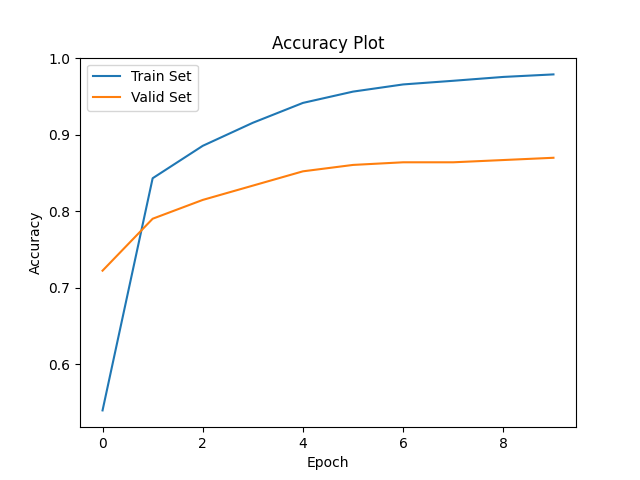
\includegraphics[scale=0.3]{./plots/supcon_10_Accuracy.png} }}
    \subfloat[\centering SimCLR]
    {{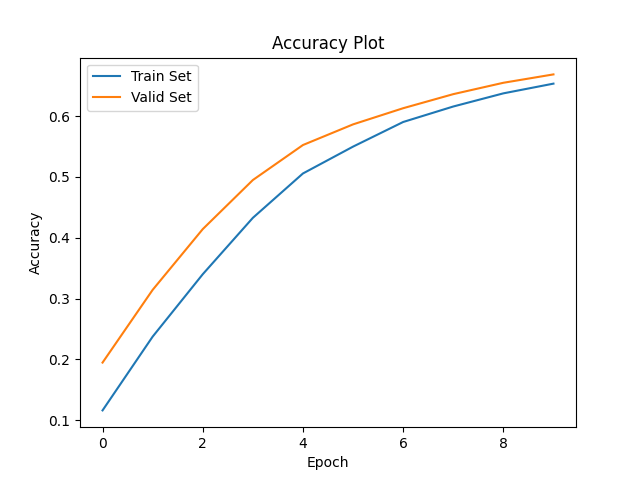
\includegraphics[scale=0.3]{./plots/supcon_sim_10_Accuracy.png} }}
\end{figure}